\documentclass[a4paper,10pt]{article}
%\documentclass[a4paper,10pt]{scrartcl}
\usepackage{multirow}
\usepackage{graphicx}
\usepackage{amsmath}
\usepackage{amsfonts}
\usepackage{amssymb}
\usepackage{xeCJK}
\usepackage[utf8]{inputenc}

\title{题解}
\date{\today}


\begin{document}
	\maketitle
	\section{energy}
      
      题目其实就是一个二维的权重矩阵在原格点图上扫描,看哪里点乘起来最大,这是经典的二维卷积。
      只要把原来的二维数组左右加0,然后拉直成一维数组,再把二维权重矩阵也拉直,就变成了一维卷积,用你们最喜爱的FFT就可以求出答案了。
      
	\section{ernd}
	
	\begin{figure}[h]
		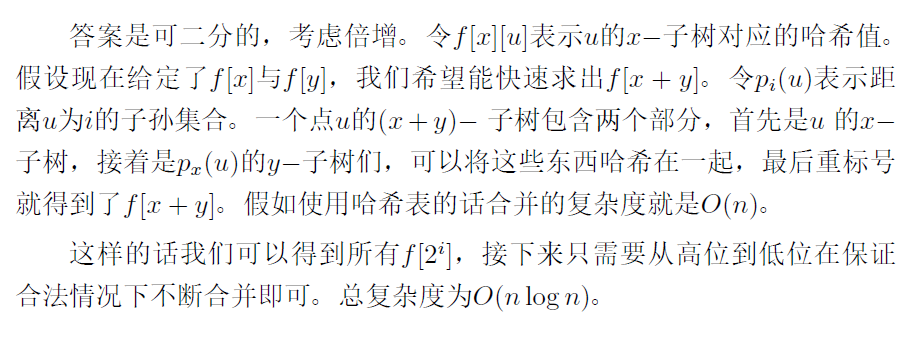
\includegraphics[width=\linewidth]{ernd_sol.png}
	\end{figure}
	
	\section{gene}
		这是2017年集训队互测题,题解参见gene.pdf.
	
\end{document}
